\PassOptionsToPackage{unicode=true}{hyperref} % options for packages loaded elsewhere
\PassOptionsToPackage{hyphens}{url}
%
\documentclass[]{article}
\usepackage{lmodern}
\usepackage{amssymb,amsmath}
\usepackage{ifxetex,ifluatex}
\usepackage{fixltx2e} % provides \textsubscript
\ifnum 0\ifxetex 1\fi\ifluatex 1\fi=0 % if pdftex
  \usepackage[T1]{fontenc}
  \usepackage[utf8]{inputenc}
  \usepackage{textcomp} % provides euro and other symbols
\else % if luatex or xelatex
  \usepackage{unicode-math}
  \defaultfontfeatures{Ligatures=TeX,Scale=MatchLowercase}
\fi
% use upquote if available, for straight quotes in verbatim environments
\IfFileExists{upquote.sty}{\usepackage{upquote}}{}
% use microtype if available
\IfFileExists{microtype.sty}{%
\usepackage[]{microtype}
\UseMicrotypeSet[protrusion]{basicmath} % disable protrusion for tt fonts
}{}
\IfFileExists{parskip.sty}{%
\usepackage{parskip}
}{% else
\setlength{\parindent}{0pt}
\setlength{\parskip}{6pt plus 2pt minus 1pt}
}
\usepackage{hyperref}
\hypersetup{
            pdftitle={SDS 323: Exercises 1 Report},
            pdfauthor={Nikhil Ajjarapu; Nevyn Duarte; Rithvik Saravanan},
            pdfborder={0 0 0},
            breaklinks=true}
\urlstyle{same}  % don't use monospace font for urls
\usepackage[margin=1in]{geometry}
\usepackage{color}
\usepackage{fancyvrb}
\newcommand{\VerbBar}{|}
\newcommand{\VERB}{\Verb[commandchars=\\\{\}]}
\DefineVerbatimEnvironment{Highlighting}{Verbatim}{commandchars=\\\{\}}
% Add ',fontsize=\small' for more characters per line
\usepackage{framed}
\definecolor{shadecolor}{RGB}{248,248,248}
\newenvironment{Shaded}{\begin{snugshade}}{\end{snugshade}}
\newcommand{\AlertTok}[1]{\textcolor[rgb]{0.94,0.16,0.16}{#1}}
\newcommand{\AnnotationTok}[1]{\textcolor[rgb]{0.56,0.35,0.01}{\textbf{\textit{#1}}}}
\newcommand{\AttributeTok}[1]{\textcolor[rgb]{0.77,0.63,0.00}{#1}}
\newcommand{\BaseNTok}[1]{\textcolor[rgb]{0.00,0.00,0.81}{#1}}
\newcommand{\BuiltInTok}[1]{#1}
\newcommand{\CharTok}[1]{\textcolor[rgb]{0.31,0.60,0.02}{#1}}
\newcommand{\CommentTok}[1]{\textcolor[rgb]{0.56,0.35,0.01}{\textit{#1}}}
\newcommand{\CommentVarTok}[1]{\textcolor[rgb]{0.56,0.35,0.01}{\textbf{\textit{#1}}}}
\newcommand{\ConstantTok}[1]{\textcolor[rgb]{0.00,0.00,0.00}{#1}}
\newcommand{\ControlFlowTok}[1]{\textcolor[rgb]{0.13,0.29,0.53}{\textbf{#1}}}
\newcommand{\DataTypeTok}[1]{\textcolor[rgb]{0.13,0.29,0.53}{#1}}
\newcommand{\DecValTok}[1]{\textcolor[rgb]{0.00,0.00,0.81}{#1}}
\newcommand{\DocumentationTok}[1]{\textcolor[rgb]{0.56,0.35,0.01}{\textbf{\textit{#1}}}}
\newcommand{\ErrorTok}[1]{\textcolor[rgb]{0.64,0.00,0.00}{\textbf{#1}}}
\newcommand{\ExtensionTok}[1]{#1}
\newcommand{\FloatTok}[1]{\textcolor[rgb]{0.00,0.00,0.81}{#1}}
\newcommand{\FunctionTok}[1]{\textcolor[rgb]{0.00,0.00,0.00}{#1}}
\newcommand{\ImportTok}[1]{#1}
\newcommand{\InformationTok}[1]{\textcolor[rgb]{0.56,0.35,0.01}{\textbf{\textit{#1}}}}
\newcommand{\KeywordTok}[1]{\textcolor[rgb]{0.13,0.29,0.53}{\textbf{#1}}}
\newcommand{\NormalTok}[1]{#1}
\newcommand{\OperatorTok}[1]{\textcolor[rgb]{0.81,0.36,0.00}{\textbf{#1}}}
\newcommand{\OtherTok}[1]{\textcolor[rgb]{0.56,0.35,0.01}{#1}}
\newcommand{\PreprocessorTok}[1]{\textcolor[rgb]{0.56,0.35,0.01}{\textit{#1}}}
\newcommand{\RegionMarkerTok}[1]{#1}
\newcommand{\SpecialCharTok}[1]{\textcolor[rgb]{0.00,0.00,0.00}{#1}}
\newcommand{\SpecialStringTok}[1]{\textcolor[rgb]{0.31,0.60,0.02}{#1}}
\newcommand{\StringTok}[1]{\textcolor[rgb]{0.31,0.60,0.02}{#1}}
\newcommand{\VariableTok}[1]{\textcolor[rgb]{0.00,0.00,0.00}{#1}}
\newcommand{\VerbatimStringTok}[1]{\textcolor[rgb]{0.31,0.60,0.02}{#1}}
\newcommand{\WarningTok}[1]{\textcolor[rgb]{0.56,0.35,0.01}{\textbf{\textit{#1}}}}
\usepackage{graphicx,grffile}
\makeatletter
\def\maxwidth{\ifdim\Gin@nat@width>\linewidth\linewidth\else\Gin@nat@width\fi}
\def\maxheight{\ifdim\Gin@nat@height>\textheight\textheight\else\Gin@nat@height\fi}
\makeatother
% Scale images if necessary, so that they will not overflow the page
% margins by default, and it is still possible to overwrite the defaults
% using explicit options in \includegraphics[width, height, ...]{}
\setkeys{Gin}{width=\maxwidth,height=\maxheight,keepaspectratio}
\setlength{\emergencystretch}{3em}  % prevent overfull lines
\providecommand{\tightlist}{%
  \setlength{\itemsep}{0pt}\setlength{\parskip}{0pt}}
\setcounter{secnumdepth}{0}
% Redefines (sub)paragraphs to behave more like sections
\ifx\paragraph\undefined\else
\let\oldparagraph\paragraph
\renewcommand{\paragraph}[1]{\oldparagraph{#1}\mbox{}}
\fi
\ifx\subparagraph\undefined\else
\let\oldsubparagraph\subparagraph
\renewcommand{\subparagraph}[1]{\oldsubparagraph{#1}\mbox{}}
\fi

% set default figure placement to htbp
\makeatletter
\def\fps@figure{htbp}
\makeatother


\title{SDS 323: Exercises 1 Report}
\author{Nikhil Ajjarapu \and Nevyn Duarte \and Rithvik Saravanan}
\date{February 14, 2020}

\begin{document}
\maketitle

\hypertarget{data-visualization-flights-at-abia}{%
\section{Data visualization: flights at
ABIA}\label{data-visualization-flights-at-abia}}

From the \texttt{ABIA.csv} data set, we could observe several
interesting patterns in the airline data at ABIA in 2008. Some of the
factors that we explored included delay caused by unique carriers, delay
caused by destination and destination weather, flight activity over time
throughout the year,

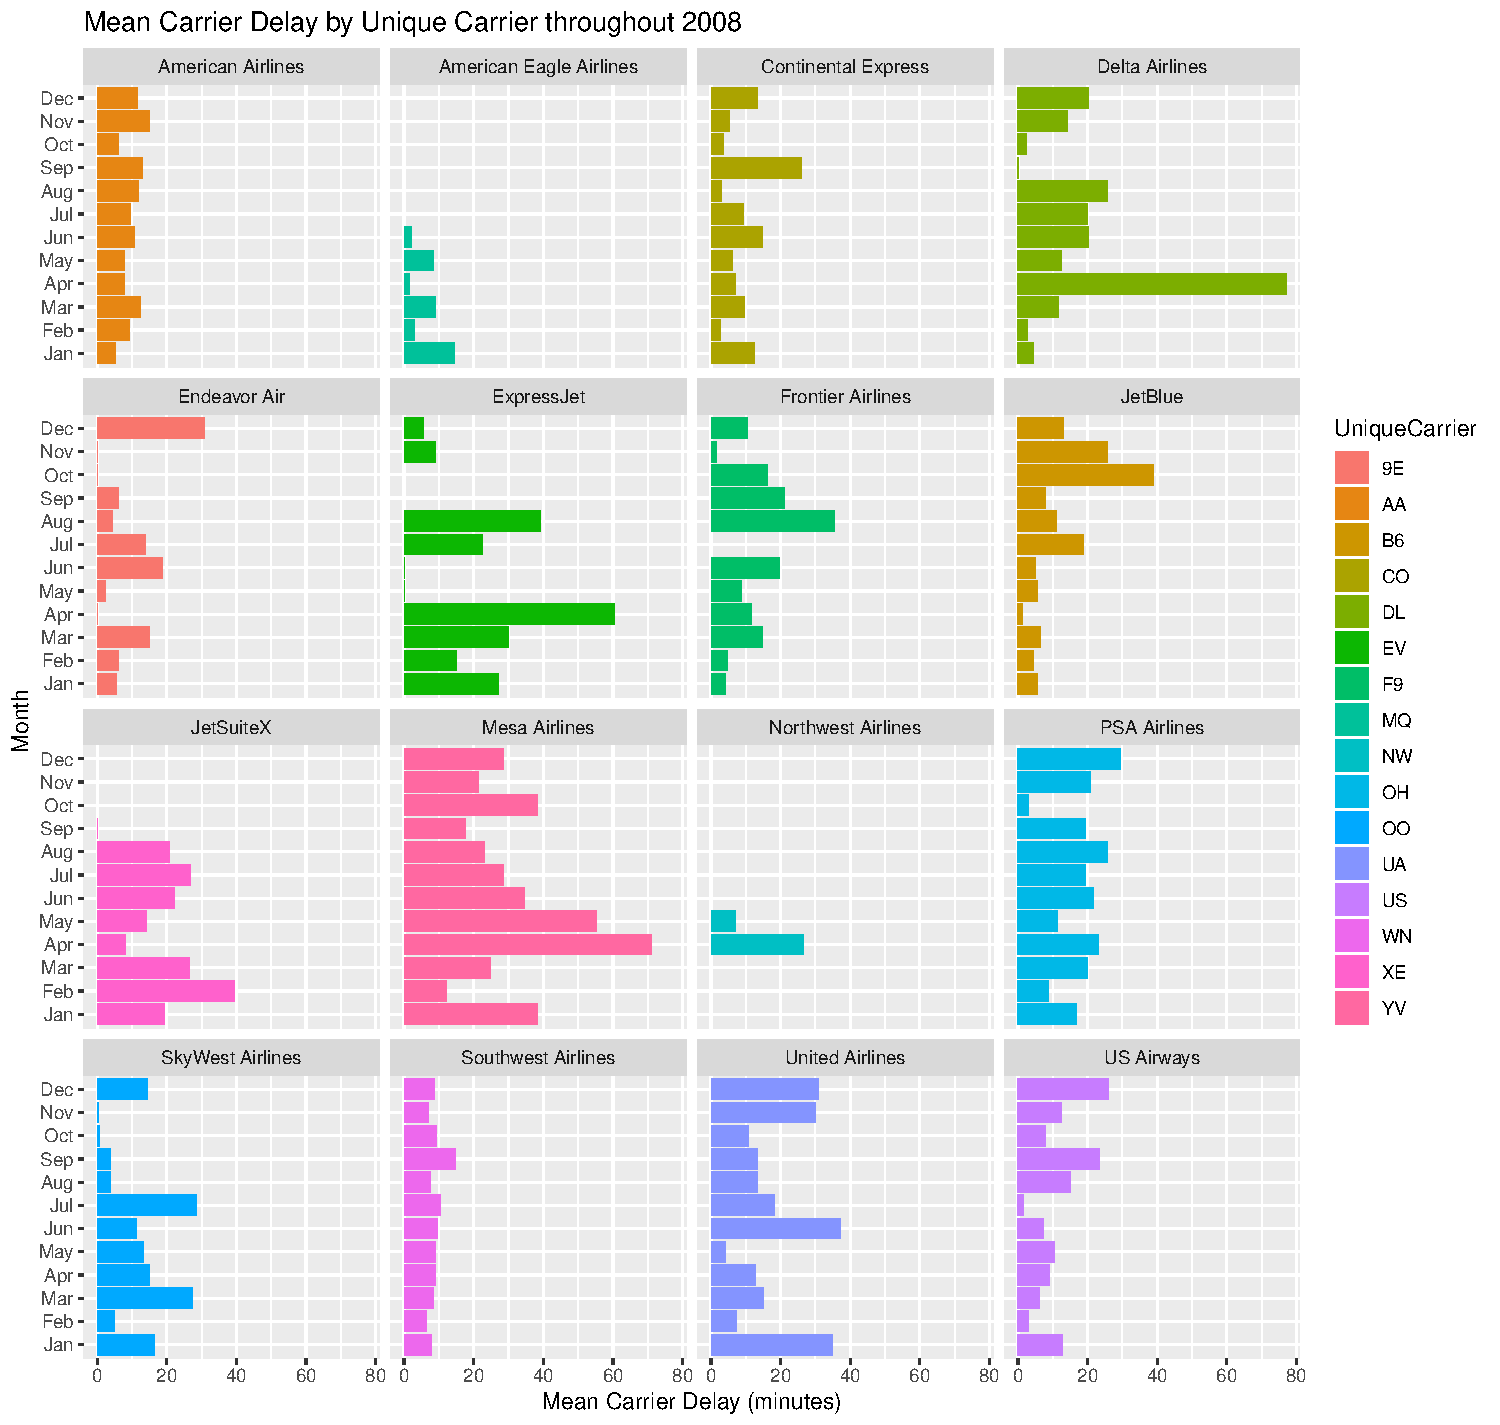
\includegraphics{Report_files/figure-latex/abia2-1.pdf}

One of the plots that we found interesting is shown above. This figure
displays the mean carrier delay by month in 2008 faceted by unique
carrier. We can see that prominent airlines such as American Airlines
and Southwest Airlines have a relatively constant and low mean carrier
delay throughout the year. This is reasonable because they are some of
the most dominant carriers at ABIA, so they likely have sufficient
staffing and resources to ensure that any flight delays are minimized.
By contrast, Mes Airlines has relatively high mean carrier delays
throughout the year, with April being the longest mean delay. Since this
carrier is less prominent at ABIA, it is logical that they would have a
limited number of flight staff and resources, which means they would not
be capable of minimizing flight delays. Another interesting point that
we notice here is that Delta Airlines had a significant jump in mean
carrier delay in the month of April. Upon further research, I learned
that there was a major breakdown at ATL (Hartsfield-Jackson Atlanta
International Airport), which is the airline hub for Delta Airlines.
According to CNN
(\url{http://www.cnn.com/2008/TRAVEL/08/26/faa.computer.failure/index.html}),
Delta Airlines and other ATL-based airlines experienced hours of flight
delays after a communications breakdown at a Federal Aviation
Administration (FAA) facility in April 2008. This communications
breakdown likely caused the significant spike mean delay in April for
Delta Airlines, especially since communications issues mean that flights
cannot depart until all safety procedures have been completed.

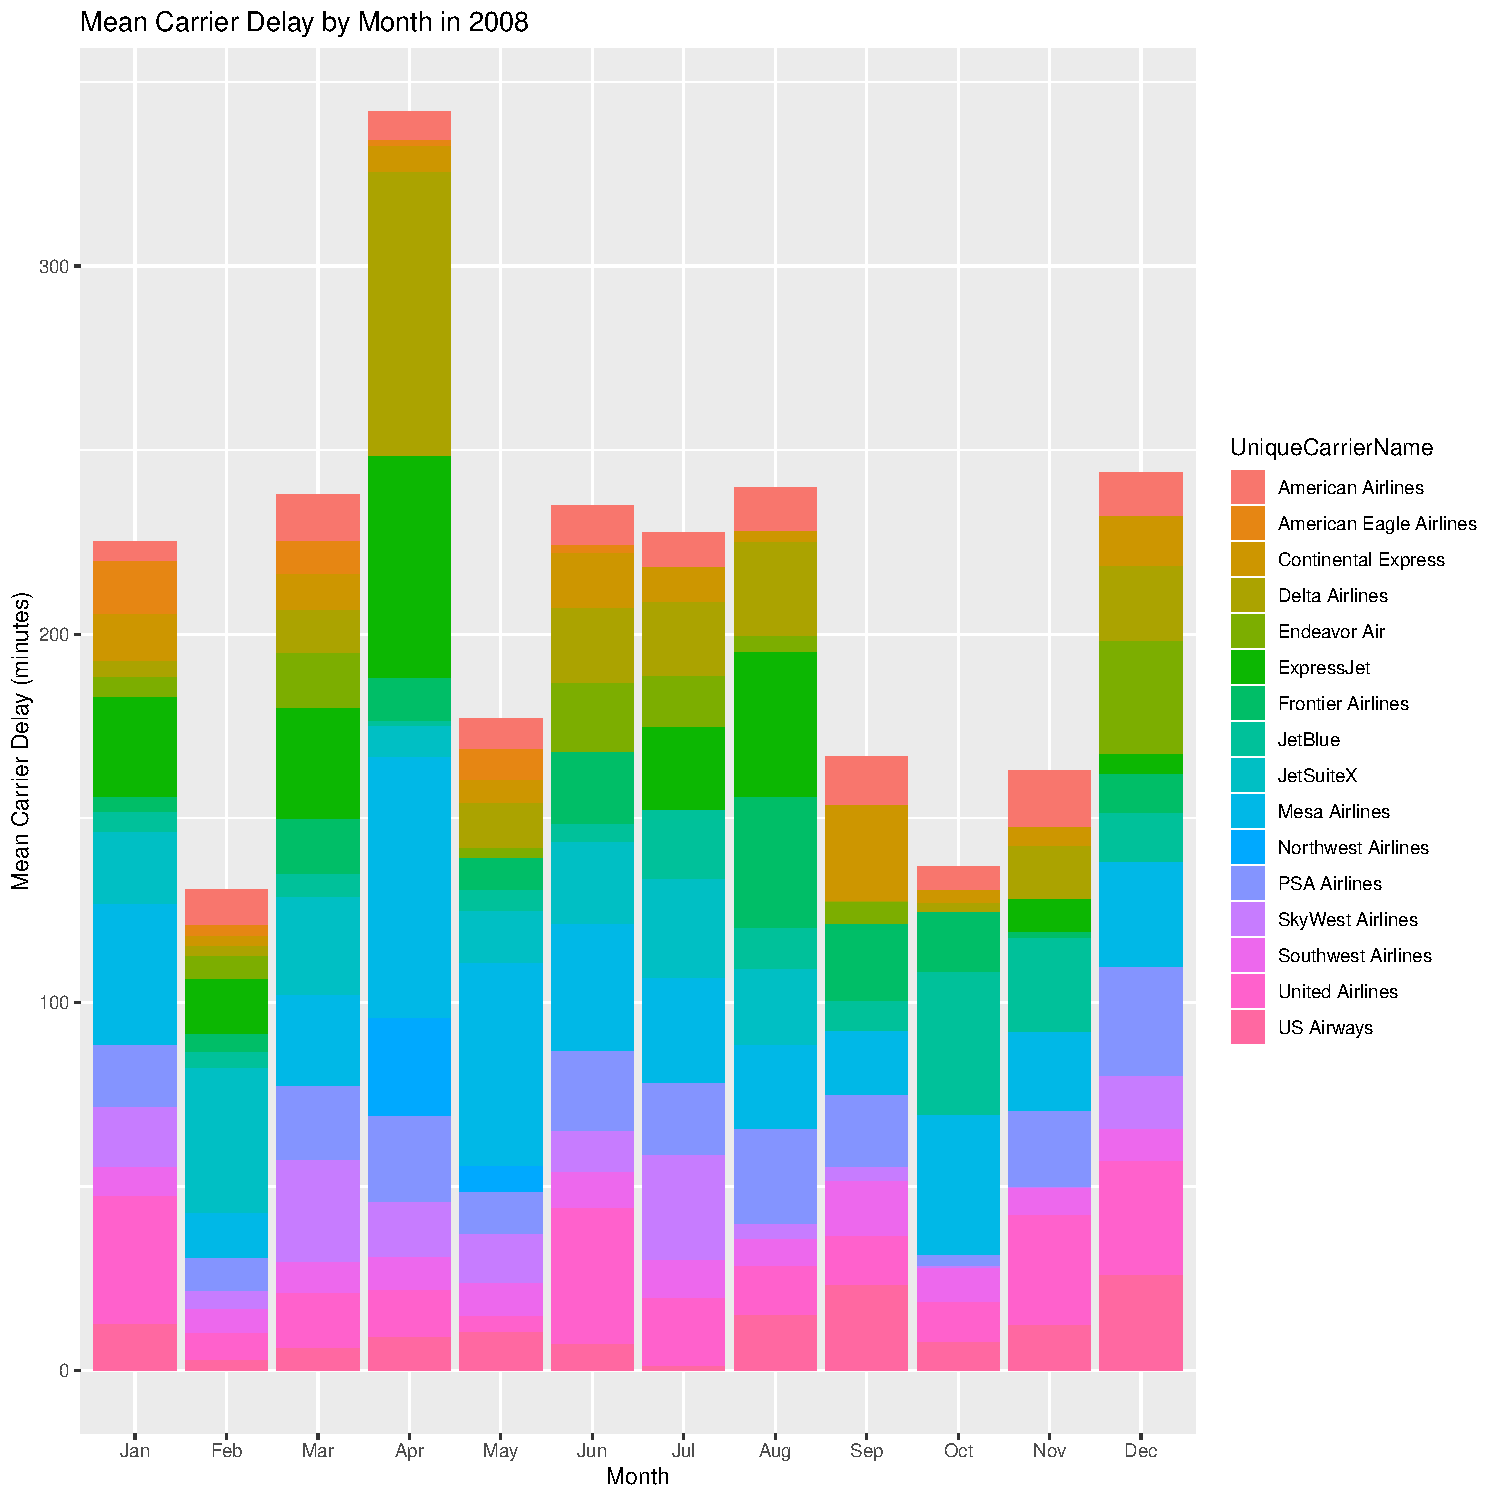
\includegraphics{Report_files/figure-latex/abia3-1.pdf}

Similar to the previous figure, the above figure displays the total mean
carrier delays by month at ABIA in 2008. This figure provides useful
information because it shows that April 2008 saw an increase in mean
carrier delays for several airlines. Due to the FAA communications
breakdown mentioned earlier, it makes sense that flights arriving from
and departing to ATL were delayed, which may have propagated the delay
to other flights as well. We also notice that the summer holiday months
of June, July, and August as well as the winter holiday months of
December and January have relatively the same amount of total mean
carrier delay. This is reasonable because these months show heavy travel
numbers as families will go on vacation, indicating that each of these
months deals with approximately the same throughput. Accordingly, the
offseason months of roughly February, May, September, October, and
November all show lower total mean carrier delay because the have
comparatively less throughput during these months since there would be
less external variables that could delay flights.

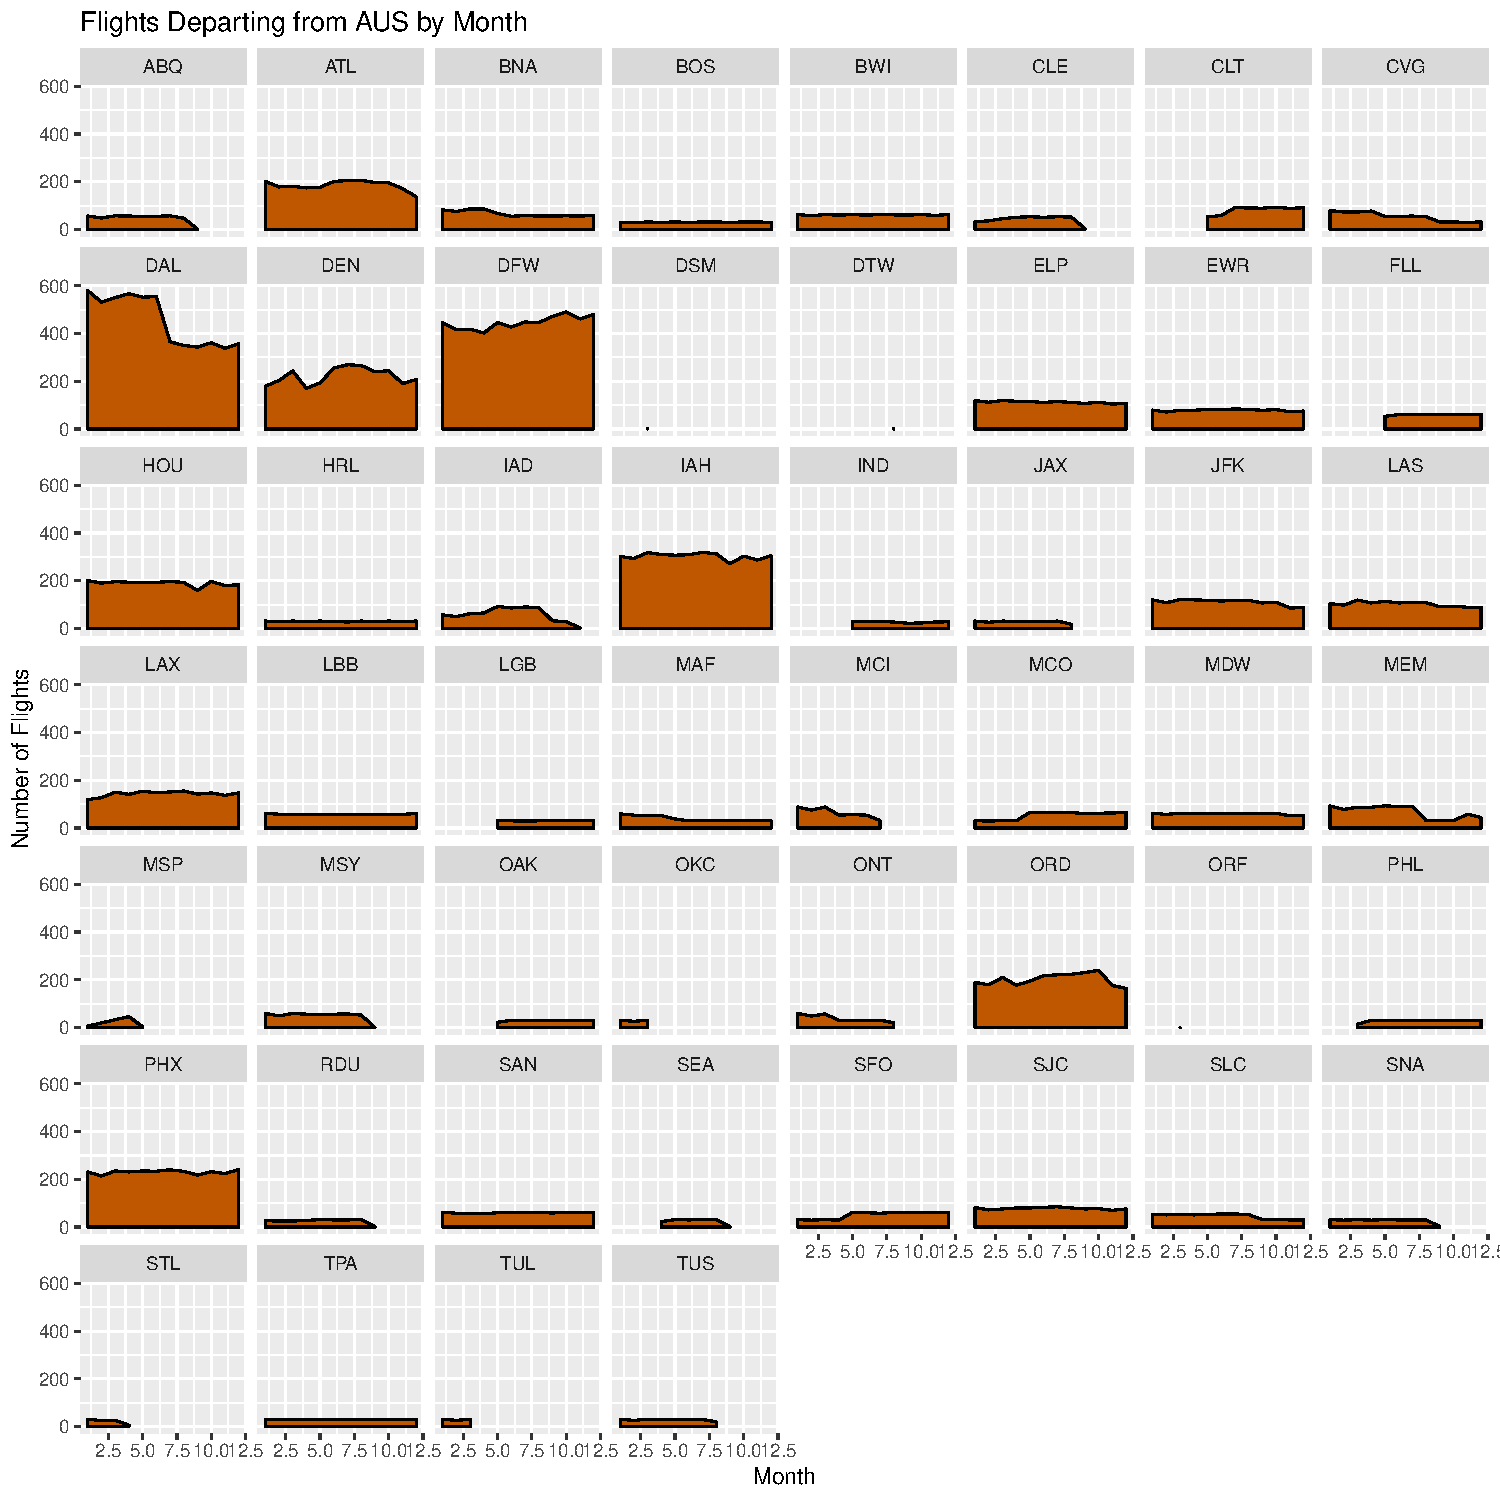
\includegraphics{Report_files/figure-latex/abia4-1.pdf}

Another intriguing figure that we came across (shown above) was showing
the number of flights departing from AUS each month in 2008 faceted by
destination airport. For airports with close geographic distance (less
than 300 miles), we can see that there were a signifiant amount of
flights consistently throughout the year. These locations include DFW,
DAL, IAH, and HOU. Additionally, the destinations that are hubs for
major airlines also had significant numbers of flights throughout the
year. For example, American Airlines has hubs in DFW and ORD, Delta
Airlines has its hub in ATL, Southwest Airlines has its hub in PHX, and
United Airlines has its hub in ORD, all of which show noticeable amounts
of flights over 2008. We also acknowledged that other destinations that
were more niche locations had seasonal variations in the number of
flights. For example, OKC only had a noticeable amount of flights in the
early portion of the year, while CLT was more popular in the later
months of the year.

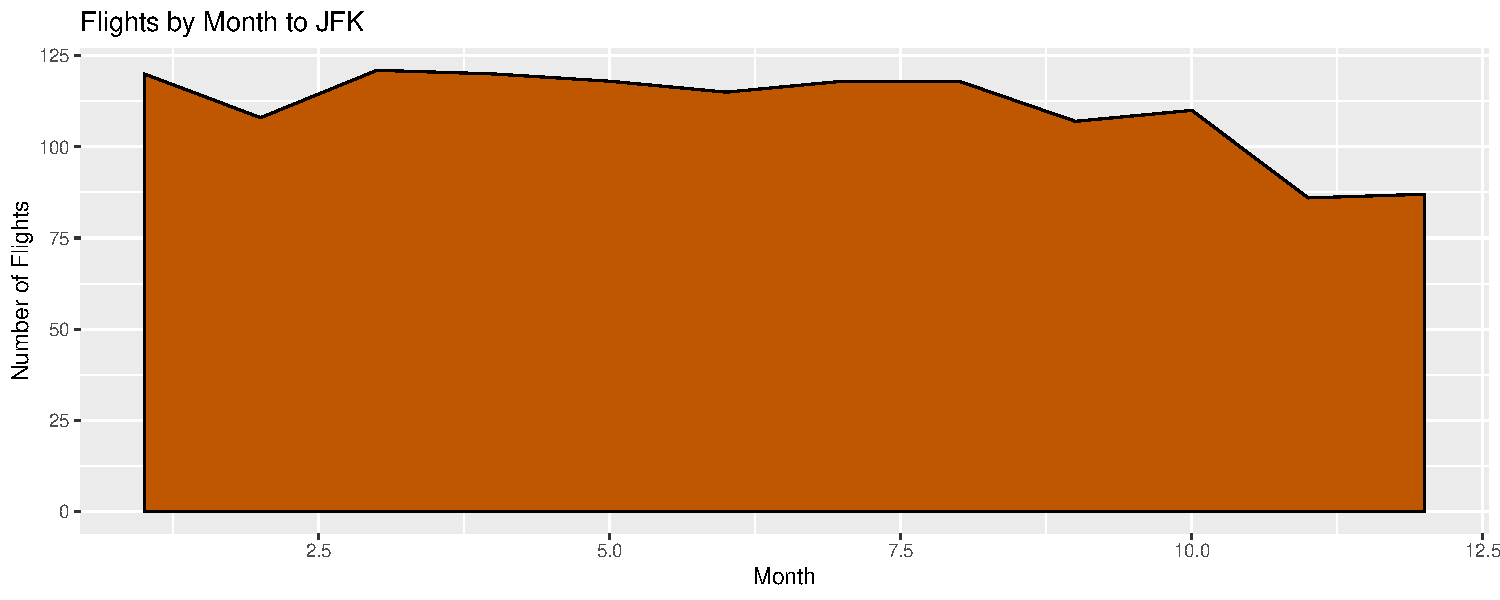
\includegraphics{Report_files/figure-latex/abia5-1.pdf}

Continuing from the previous figure, we can see that flights to JFK
dropped significantly in the months of November and December. While this
could be because those are holiday months (i.e Thanksgiving, Christmas,
etc.) and less people are traveling to New York for business-related
matters, I believe that this phenomenon was due to the financial crisis
in 2008. Due to the severe recession and economic downturn in 2008, it
is plausible that many people who worked in New York in the business
industry (like Wall Street) were laid off from their jobs.\n

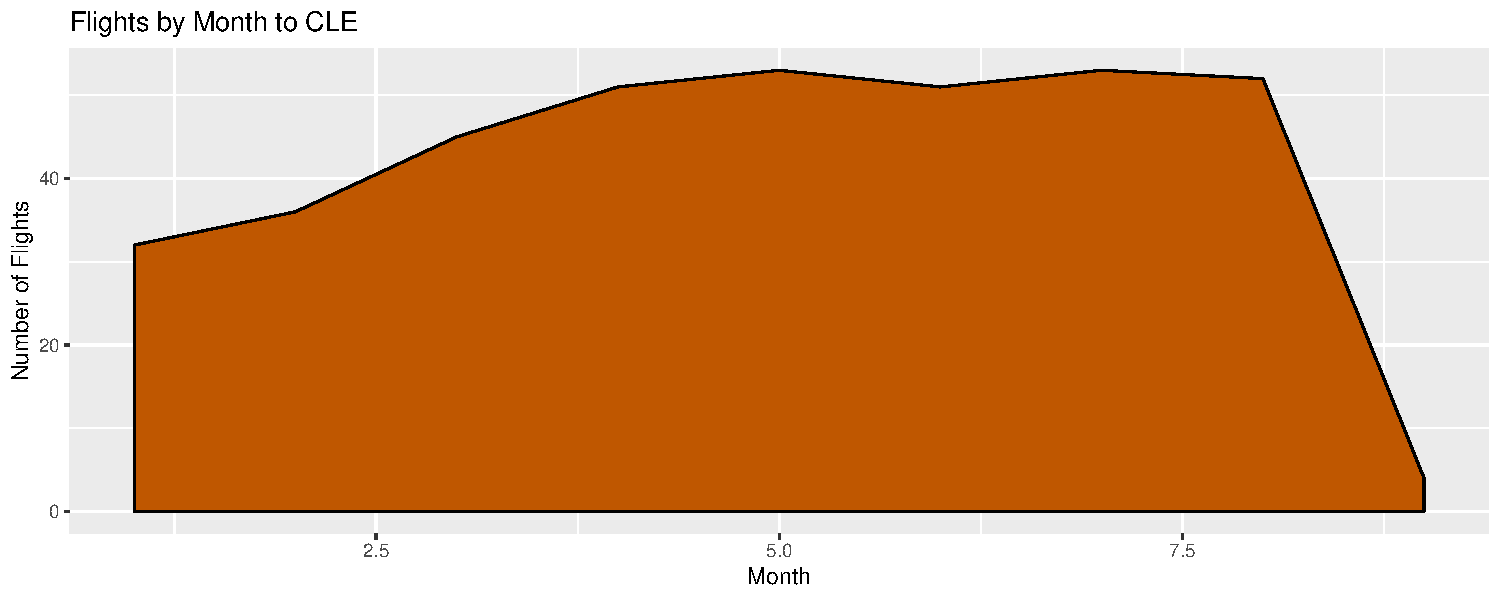
\includegraphics{Report_files/figure-latex/abia6-1.pdf}

Another extension of the 3rd figure, we noticed that there were
significantly fewer flights to CLE in the months of January, February,
and March. Upon further research
(\url{https://www.weather.gov/cle/event_2008_notable}), we identified
that February and March gathered most of the monthly precipitation
records for 2008 for Cleveland, Ohio. Accordingly, this density plot
shows that there were noticeably fewer flights to CLE in the months of
February and March compared to the following months. Due to the
inclement weather during these early months, it is logical that fewer
flights were scheduled for Cleveland.

\hypertarget{regression-practice}{%
\section{Regression practice}\label{regression-practice}}

Using the data given in \texttt{creatinine.csv}, we can plot the values
in a scatterplot that shows creatinine clearance rate against age. On
this scatterplot, we can fit a linear model as the line of best fit.
This linear regression model will allow us to predict creatinine
clearance rate given age and vice versa. The scatterplot and the
coefficients of the linear model are given below.

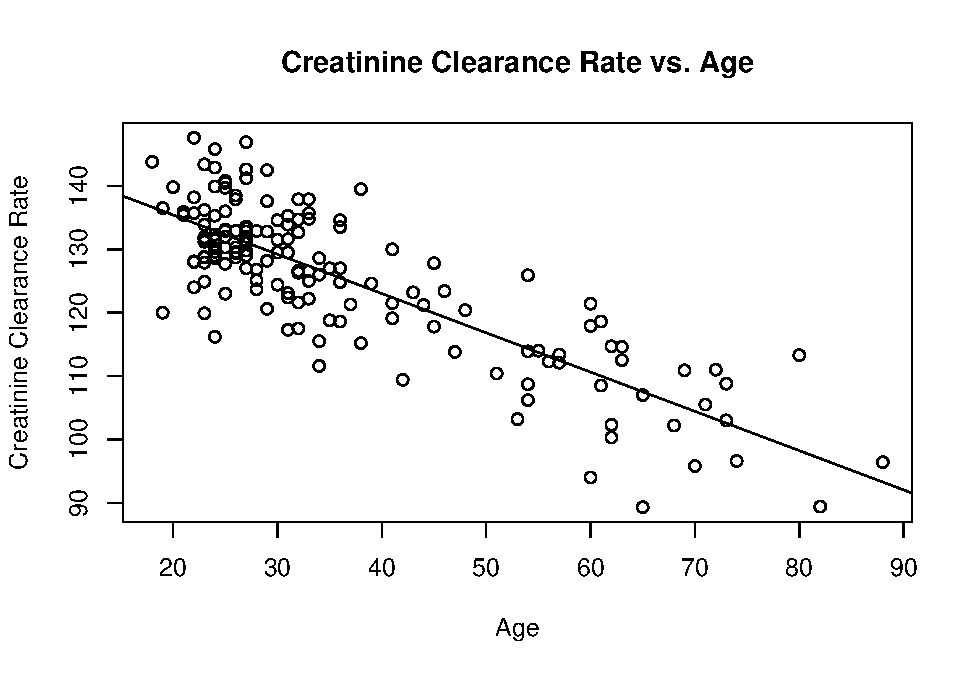
\includegraphics{Report_files/figure-latex/creatinine2-1.pdf}

\begin{verbatim}
## (Intercept)         age 
## 147.8129158  -0.6198159
\end{verbatim}

The slope coefficient (shown as \texttt{age} above) of the linear model
indicates that the creatinine clearance rate decreases by 0.6198
mL/minute per year. This is a reasonable rate of change because we know
that a higher creatinine clearance rate is better and that it should
generally decrease as age increases.

From the linear regression model, we can also compute the residuals for
each of the data points and plot them on a residual plot as shown below.

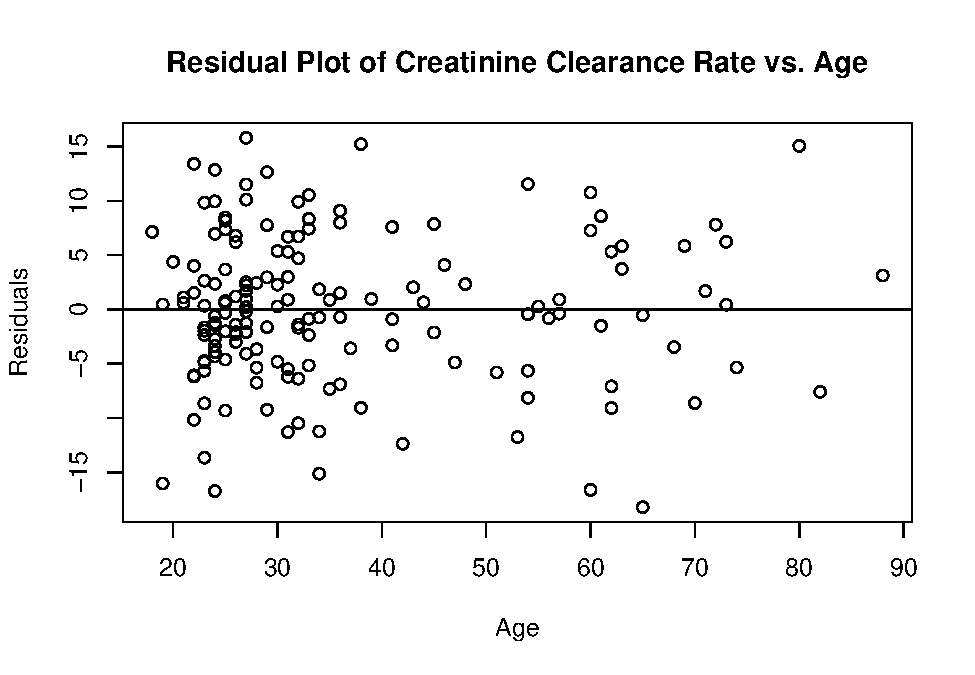
\includegraphics{Report_files/figure-latex/creatinine3-1.pdf}

We can also interpolate new data points to predict their values:

\begin{Shaded}
\begin{Highlighting}[]
\CommentTok{# make prediction on new data}
\NormalTok{new_data =}\StringTok{ }\KeywordTok{data.frame}\NormalTok{(}\DataTypeTok{age =} \KeywordTok{c}\NormalTok{(}\DecValTok{55}\NormalTok{))}
\KeywordTok{predict}\NormalTok{(lm1, new_data)}
\end{Highlighting}
\end{Shaded}

\begin{verbatim}
##       1 
## 113.723
\end{verbatim}

Accordingly, we can see that, for an average 55-year-old, we should
expect a creatinine clearance rate of 113.723 mL/minute.

To identify whether a 40-year-old with a rate of 135 or a 60-year-old
with a rate of 112 is healthier for their respective age, we can predict
creatinine clearance rates for average people of their age and compute
the residuals.

\begin{Shaded}
\begin{Highlighting}[]
\CommentTok{# make predictions on new data to compare patients}
\NormalTok{patient_data =}\StringTok{ }\KeywordTok{data.frame}\NormalTok{(}\DataTypeTok{age =} \KeywordTok{c}\NormalTok{(}\DecValTok{40}\NormalTok{, }\DecValTok{60}\NormalTok{))}
\KeywordTok{predict}\NormalTok{(lm1, patient_data)}
\end{Highlighting}
\end{Shaded}

\begin{verbatim}
##        1        2 
## 123.0203 110.6240
\end{verbatim}

\begin{Shaded}
\begin{Highlighting}[]
\CommentTok{# compute residuals for each patient}
\DecValTok{135} \OperatorTok{-}\StringTok{ }\FloatTok{123.0203}
\end{Highlighting}
\end{Shaded}

\begin{verbatim}
## [1] 11.9797
\end{verbatim}

\begin{Shaded}
\begin{Highlighting}[]
\DecValTok{112} \OperatorTok{-}\StringTok{ }\FloatTok{110.6240}
\end{Highlighting}
\end{Shaded}

\begin{verbatim}
## [1] 1.376
\end{verbatim}

Since the 40-year-old with a rate of 135 mL/minute has a residual of
11.9797 mL/minute and the 60-year-old with a rate of 112 mL/minute has a
residual of 1.376 mL/minute, the 40-year-old has a healthier creatinine
clearance rate. This is because a higher positive residual value is
considered to indicate better health since it means that the actual rate
of the 40-year-old subject is much greater than the predicted rate for
40-year-olds while the actual rate of the 60-year-old subject is only
slightly greater than the predicted rates for 60-year-olds.

\hypertarget{green-buildings}{%
\section{Green buildings}\label{green-buildings}}

In order to aid the Austin real-estate developer in determining the
possible economic impact of ``going green'' and investing in a green
building, we can analyze \texttt{greenbuildings.csv} to identify whether
green building status indeed affects the rent costs of a building. If
not, we can also examine the data set to identify other potential
factors that could contribute to the rent costs of a building.

After understanding the on-staff data guru's analysis, we conclude that
their analysis is not entirely accurate, and that they fail to take into
account various confounding variables that may be better indicators of
whether a building will be profitable or not. To begin, we also filtered
out the buildings with less than 10\% occupancy, but we also filtered
out the buildings that had the \texttt{net} feature equal to 0. This
meant we were removing buildings where the tenant paid for their own
utilities because this could skew the rent that they were paying. Next,
we looked at various correlation coefficients between different features
of the data set to see if anything was more correlated to the
\texttt{Rent} feature than the \texttt{green\ rating}. We found that
\texttt{cluster\_rent} and \texttt{electricity\_costs} were each very
strongly correlated with \texttt{Rent}, with \emph{r}-values of 0.75 and
0.41, respectively. We also found that the \emph{r}-value between
\texttt{green\_rating} and \texttt{Rent} was only 0.03, indicating a
poor correlation between the two values. In addition, we created a few
plots to identify the effect of confounding variables:

\hypertarget{age}{%
\subsection{Age}\label{age}}

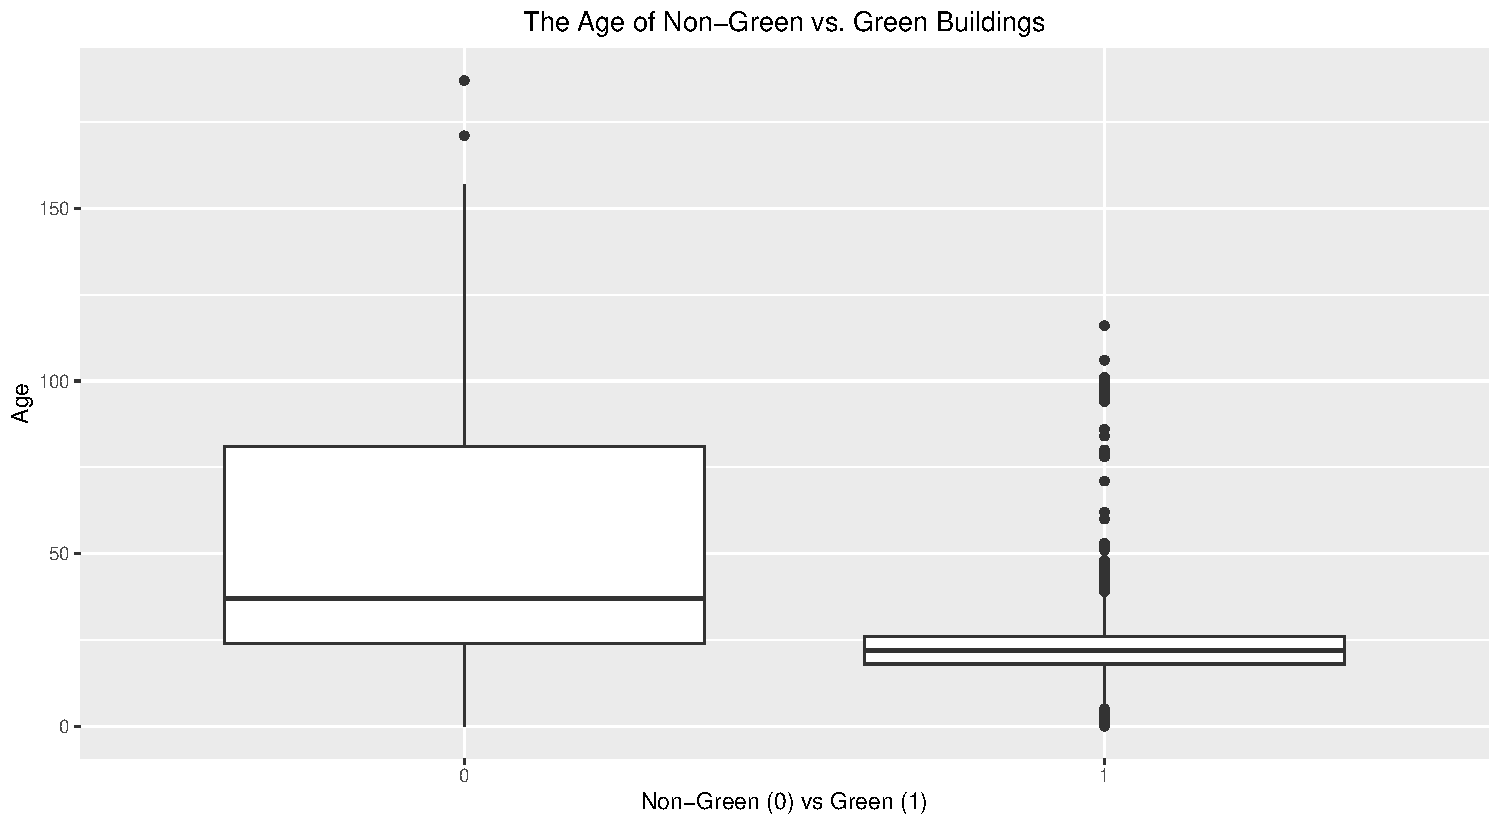
\includegraphics{Report_files/figure-latex/age_box-1.pdf}

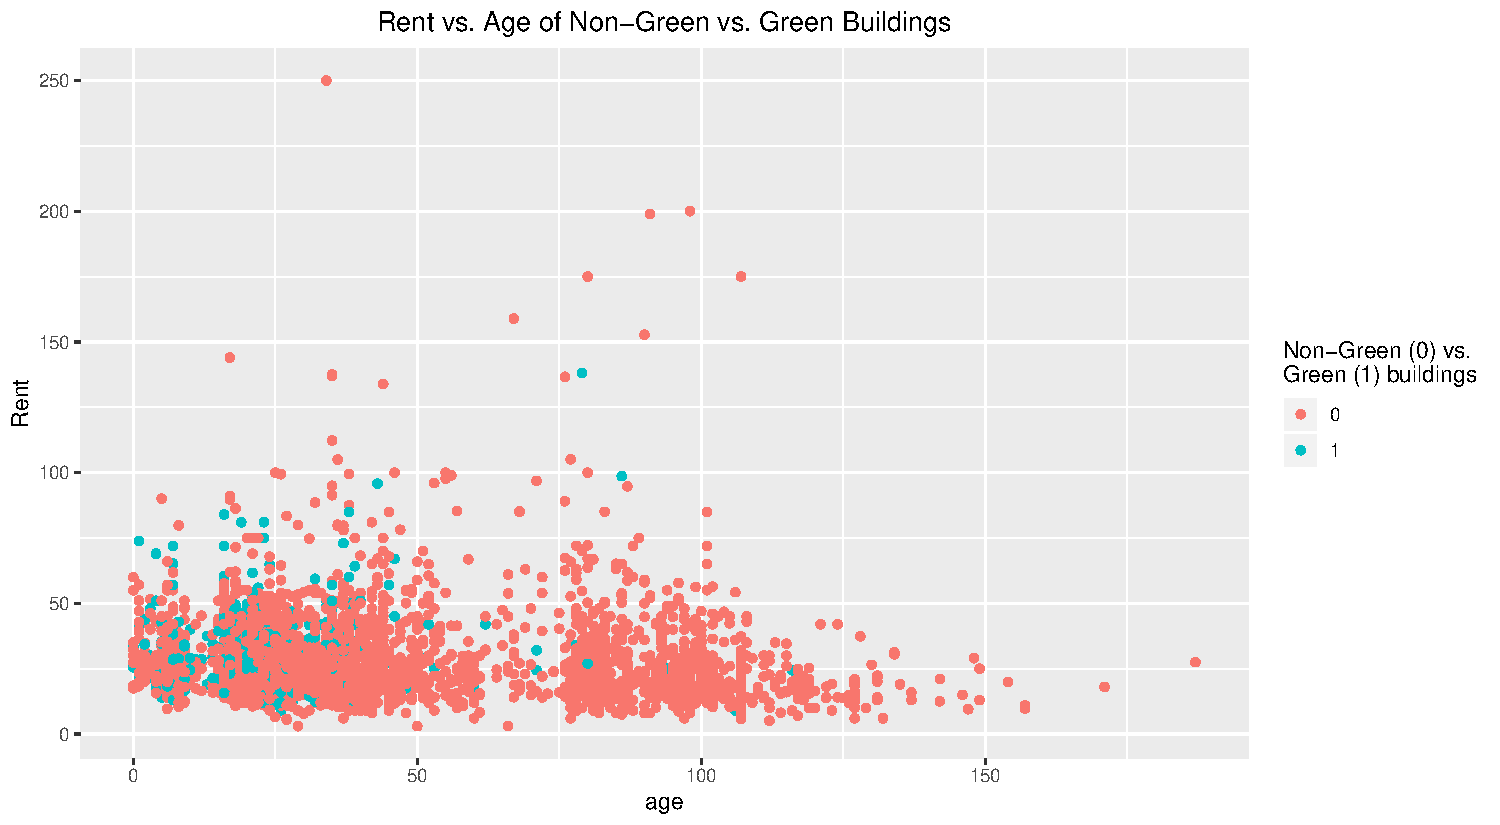
\includegraphics{Report_files/figure-latex/age_scatter-1.pdf}

The first plot shows that green buildings on average tend to be newer
(younger age) than non-green buildings. This shows that green buildings
could be more expensive and require higher rent costs because they are
more premium real estate. The second plot is a scatterplot of all the
data points plotted by rent and age, where it is apparent that the green
buildings are concentrated towards the left side of the graph,
indicating that they are generally younger than non-green buildings.

\hypertarget{cluster-rent}{%
\subsection{Cluster Rent}\label{cluster-rent}}

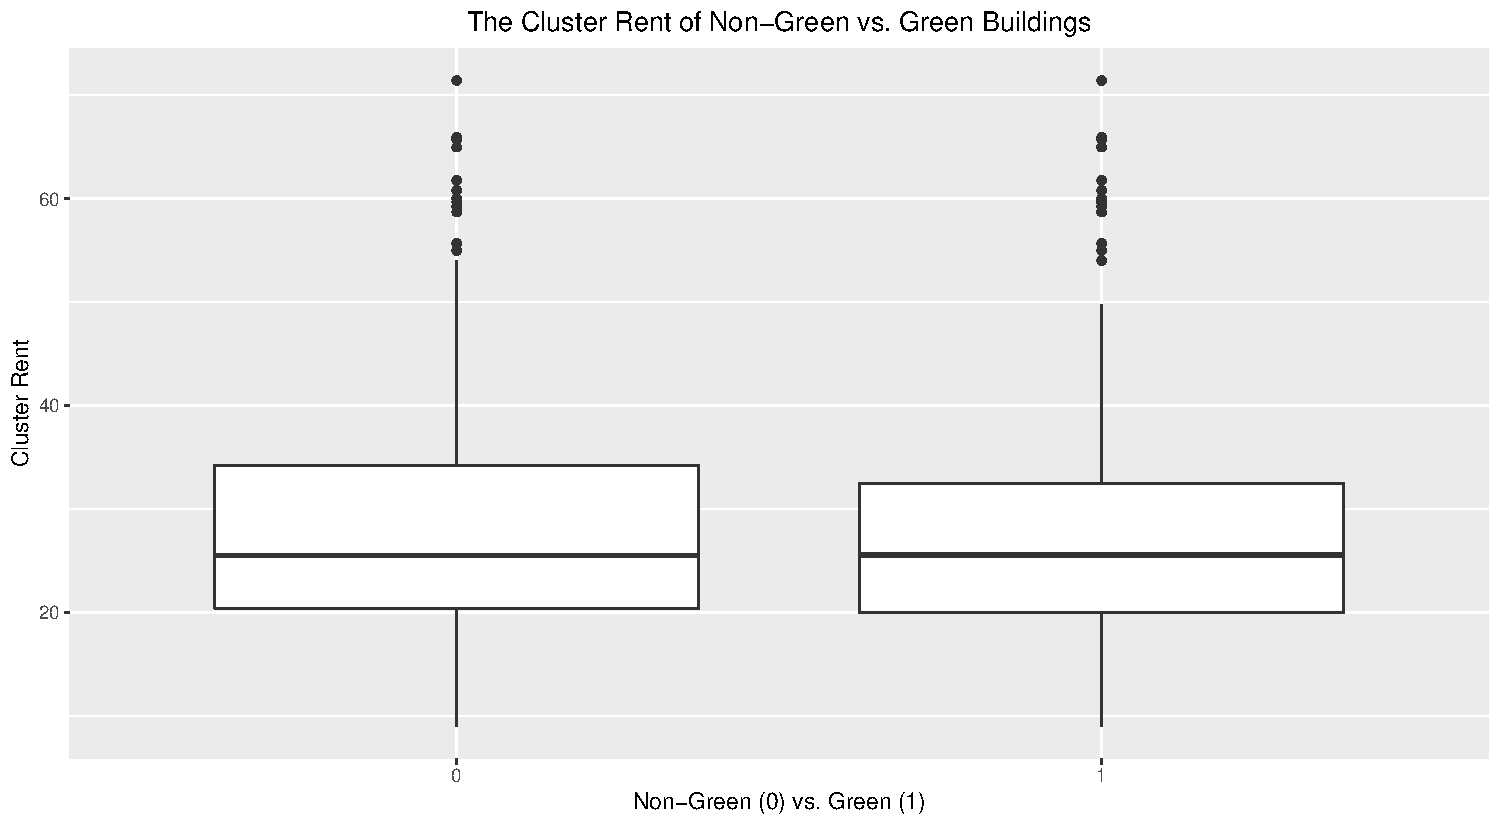
\includegraphics{Report_files/figure-latex/cluster_box-1.pdf}

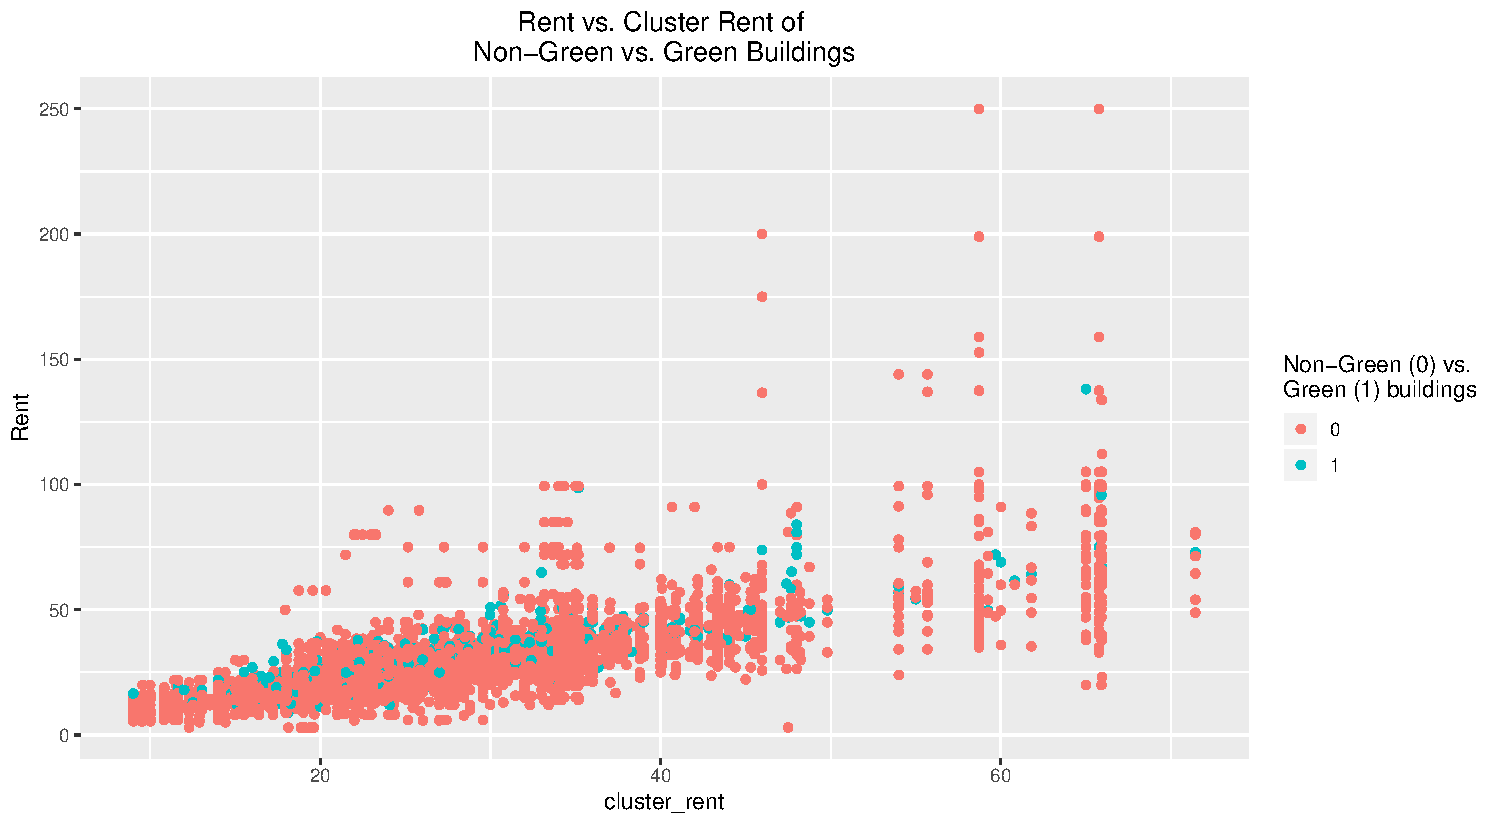
\includegraphics{Report_files/figure-latex/cluster_scatter-1.pdf}

The plot above shows that when controlled for cluster rent, it seems
that green and non-green buildings could potentially be equally
profitable. Cluster rent, as mentioned above, has the strongest
correlation to rent (evidenced by the scatterplot above), which simply
means that the rent of all the buildings in a similar geographic region
has the strongest effect on the rent of a building. If we take this
variable into account, the rents seem to be equalized. This is
reasonable because the rent costs in a metro area will generally be
higher overall than the rent costs in suburban or rural areas.

\hypertarget{electricity-costs}{%
\subsection{Electricity Costs}\label{electricity-costs}}

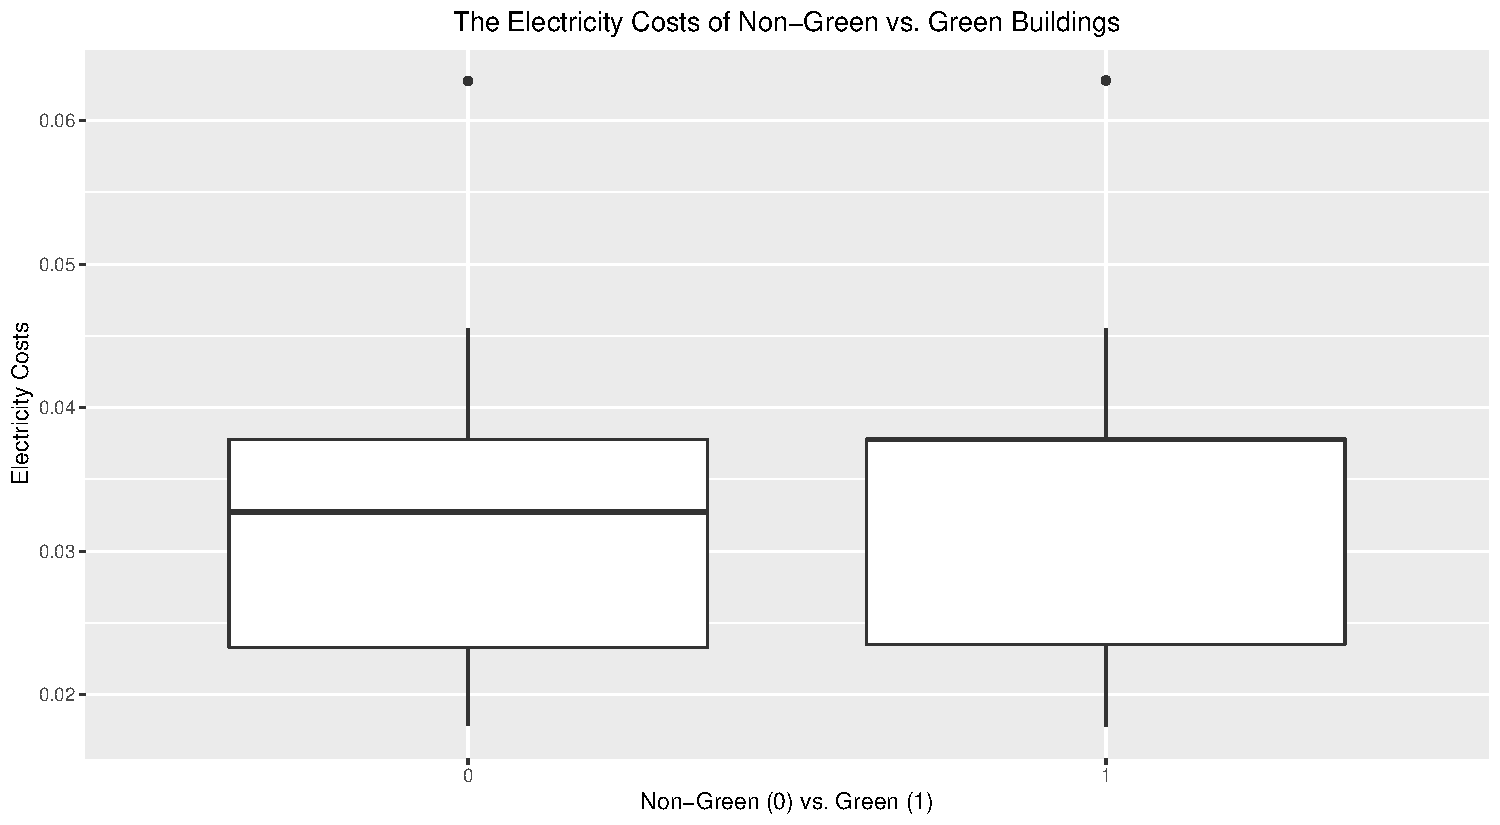
\includegraphics{Report_files/figure-latex/elec_box-1.pdf}

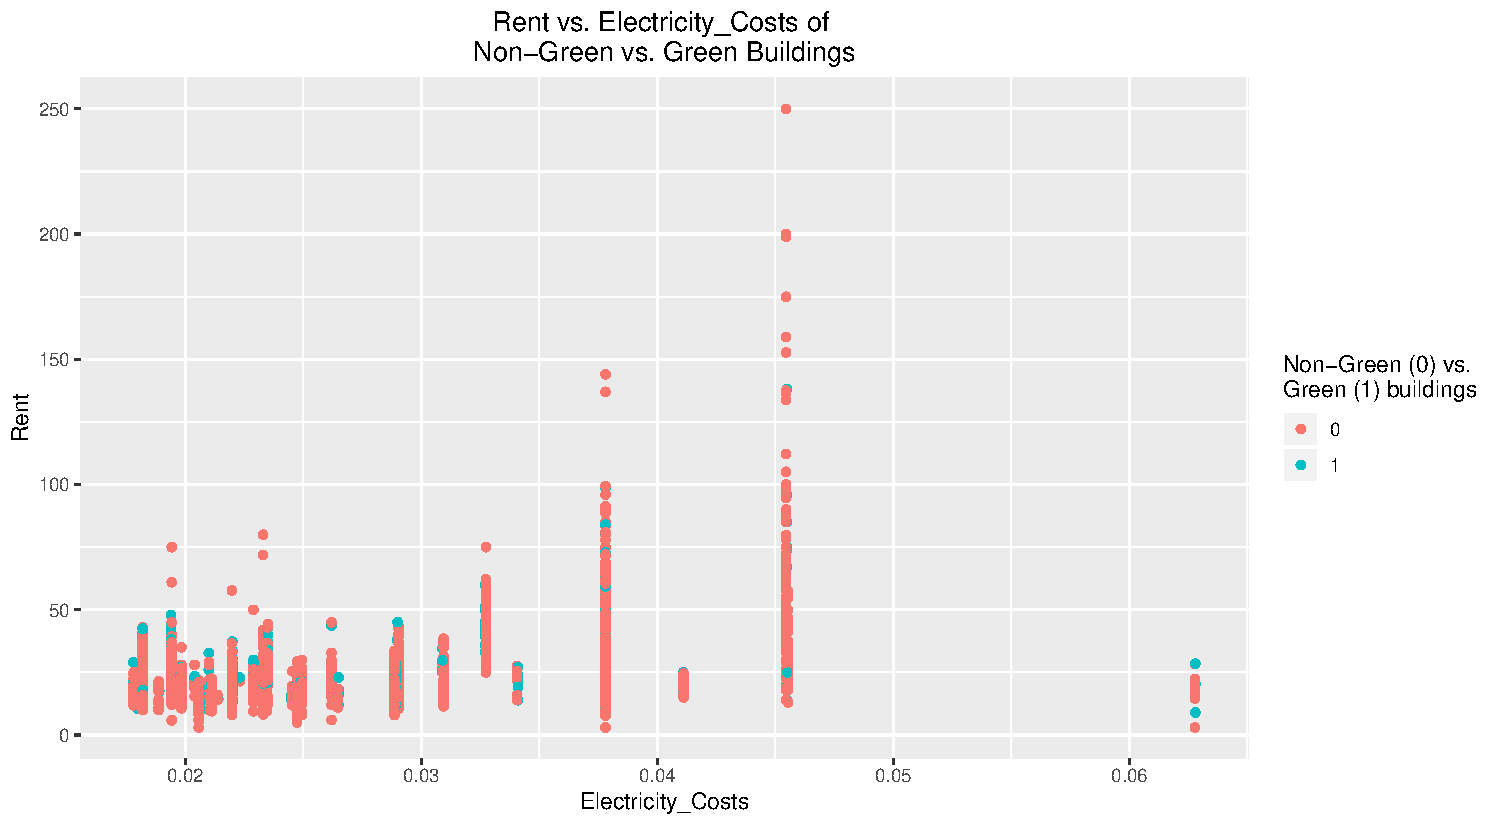
\includegraphics{Report_files/figure-latex/elec_scatter-1.pdf}

Another potential confounding variable is the electricity costs of the
area that the building is in, which was mentioned above as having the
2nd highest correlation with rent. The box plot clearly indicates that
the median electricity cost in the areas green buildings are built is
higher, which could explain the higher rent. The scatter plot also
supports this idea, with most of the blue dots (green buildings) above
the red dots (non-green buildings). The plots combined indicate that
electricity costs in the area might be a better indicator of rent,
especially as electricity costs are intrinsically tied to the concept of
green/non-green buildings.

All in all, we can see through the various different plots that
variables such as the age of the building, the mean rent of the cluster
the building is part of, and the cost of electricity in the geographic
region of the building all played an important role in determining the
rent of the building itself. We conclude that due to the sheer number of
other variables at work here that explain some of the causality and
correlation between green vs non-green buildings and higher rent, the
analysis in the case study isn't entirely accurate and is worth
revisiting. Solely building a green building for higher profits may not
result in the desired outcome, so the investor should take into account
other factors in order to make their decision.

\hypertarget{milk-prices}{%
\section{Milk prices}\label{milk-prices}}

The \texttt{milk.csv} data set includes certain days' quantity in units
of milk sold and the price it was sold for at a specific small
neighborhood grocery store. From the perspective of the merchant, we
would like to maximize the profit. To do so, we need to identify the
optimal price to sell the milk. Our profit equation for this scenario is
\(N = (P - c) \cdot Q\) where \(P\) is the selling price, \(Q\) is the
quantity sold, \(N\) is the profit, and \(c\) is the cost to buy from
wholesaler.

\begin{Shaded}
\begin{Highlighting}[]
\CommentTok{# scatterplot of sales vs price}
\KeywordTok{plot}\NormalTok{(sales }\OperatorTok{~}\StringTok{ }\NormalTok{price, }\DataTypeTok{data =}\NormalTok{ milk, }\DataTypeTok{main =} \StringTok{"Milk Sales vs. Price"}\NormalTok{,}
     \DataTypeTok{xlab =} \StringTok{"Price per Unit ($)"}\NormalTok{,}
     \DataTypeTok{ylab =} \StringTok{"Sales (units sold per day)"}\NormalTok{)}
\end{Highlighting}
\end{Shaded}

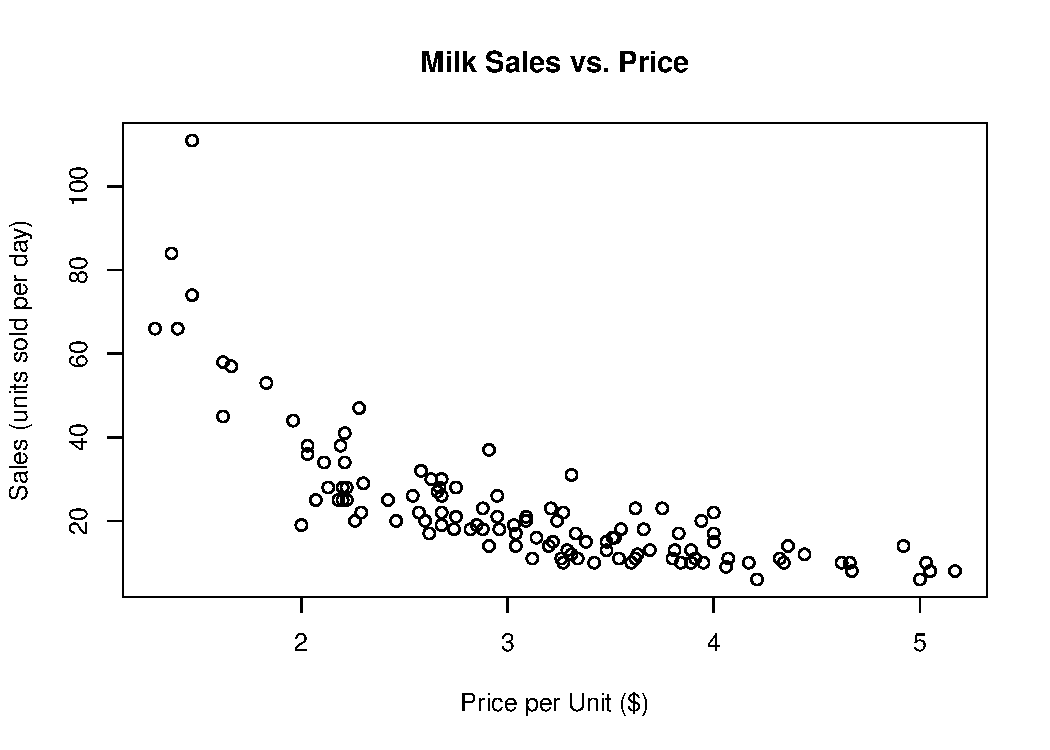
\includegraphics{Report_files/figure-latex/milk2-1.pdf}

From basic economic laws of supply and demand, we know that \(P\) and
\(Q\) are inversely related because the demand for the milk will
increase as the price decreases. Therefore, we can set \(Q = f(P)\) and
our profit equation becomes \(N = (P - c) \cdot f(P)\).

Using the Power law, we can show this as \(Q = \alpha \cdot P^\beta\)
where \(\beta\) is the price elasticity of demand and \(\alpha\) is a
constant. Taking the logarithm of both sides of the equation, we reach
\(\log (Q) = \log (\alpha) + \beta \cdot \log (P)\).

\begin{Shaded}
\begin{Highlighting}[]
\CommentTok{# scatterplot of log(sales) vs log(price)}
\KeywordTok{plot}\NormalTok{(}\KeywordTok{log}\NormalTok{(sales) }\OperatorTok{~}\StringTok{ }\KeywordTok{log}\NormalTok{(price), }\DataTypeTok{data =}\NormalTok{ milk, }\DataTypeTok{main =} \StringTok{"Milk Sales vs. Price (Log Scale)"}\NormalTok{,}
     \DataTypeTok{xlab =} \StringTok{"Log of Price per Unit ($)"}\NormalTok{,}
     \DataTypeTok{ylab =} \StringTok{"Log of Sales (units sold per day)"}\NormalTok{)}
\end{Highlighting}
\end{Shaded}

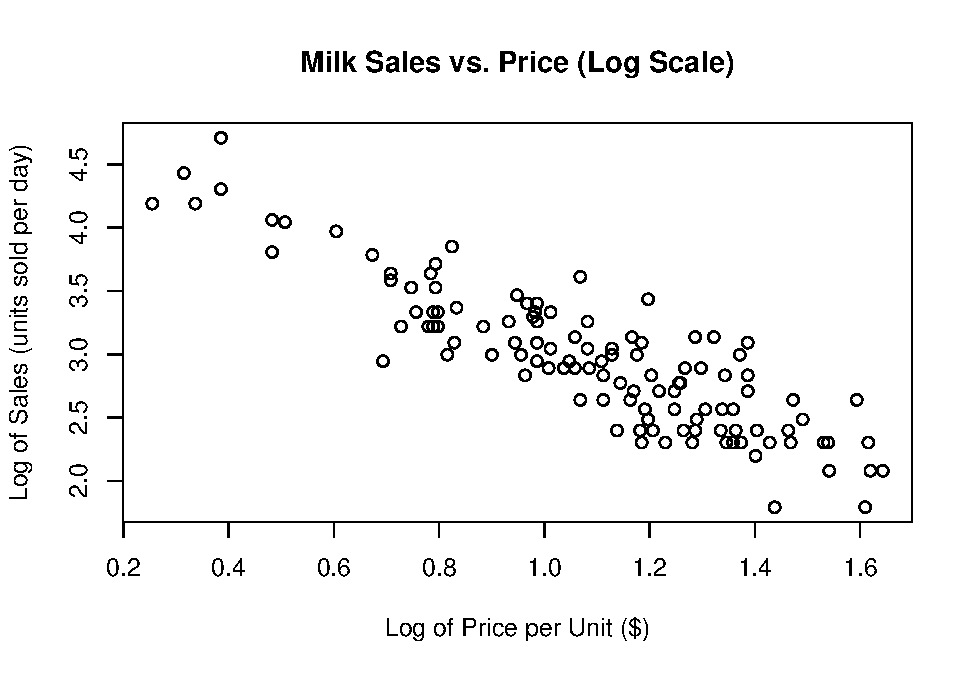
\includegraphics{Report_files/figure-latex/milk3-1.pdf}

\begin{Shaded}
\begin{Highlighting}[]
\CommentTok{# linear model for line of best fit for log scatterplot}
\NormalTok{lm_ped =}\StringTok{ }\KeywordTok{lm}\NormalTok{(}\KeywordTok{log}\NormalTok{(sales) }\OperatorTok{~}\StringTok{ }\KeywordTok{log}\NormalTok{(price), }\DataTypeTok{data =}\NormalTok{ milk)}
\KeywordTok{coef}\NormalTok{(lm_ped)}
\end{Highlighting}
\end{Shaded}

\begin{verbatim}
## (Intercept)  log(price) 
##    4.720604   -1.618578
\end{verbatim}

We can now see that the coefficients of the linear regression model are
4.720604 and -1.618578. Plugging these values in for \(\log (\alpha)\)
and \(\beta\), respectively, we get
\(\log (Q) = 4.72 - 1.62 \cdot \log (P)\). By raising both sides to the
exponent, we can remove the logarithm on the LHS and solve for \(Q\) as
\(Q = e^{4.72} \cdot P^{-1.62}\). Now that we have solved for \(Q\) as a
function of \(P\), we can plug \(Q\) back into our profit equation as
\(N = (P - c) \cdot e^{4.72} \cdot P^{-1.62}\). Computing the exponent
value gives us \(N = (P - c) \cdot 112.24 \cdot P^{-1.62}\). Since we
know that the per-unit cost \(c\) is \$1, we can plot the curve with the
equation \(N = (P - 1) \cdot 112.24 \cdot P^{-1.62}\).

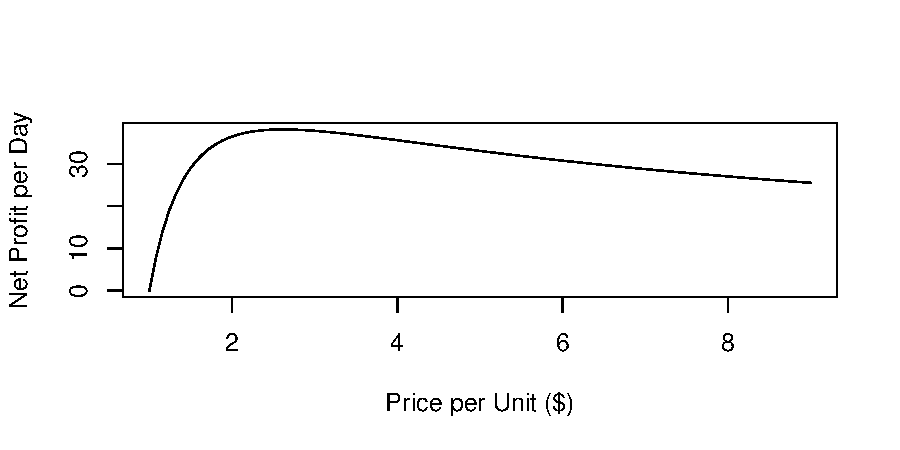
\includegraphics{Report_files/figure-latex/milk5-1.pdf}
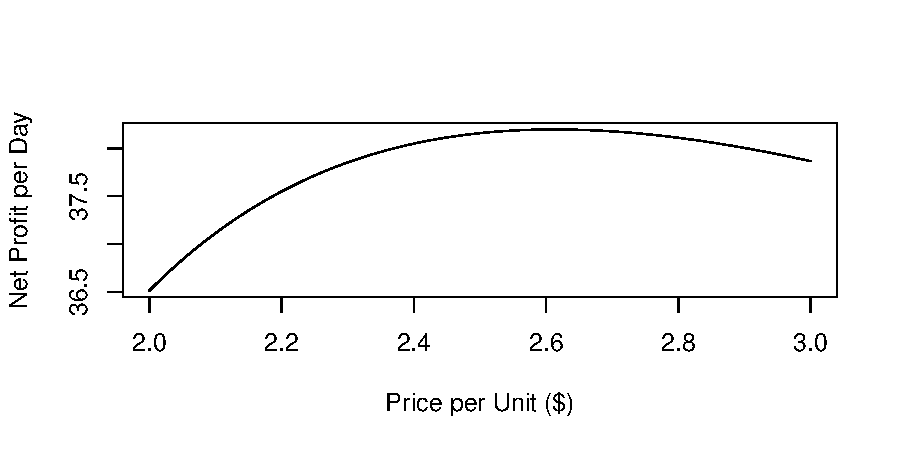
\includegraphics{Report_files/figure-latex/milk6-1.pdf}
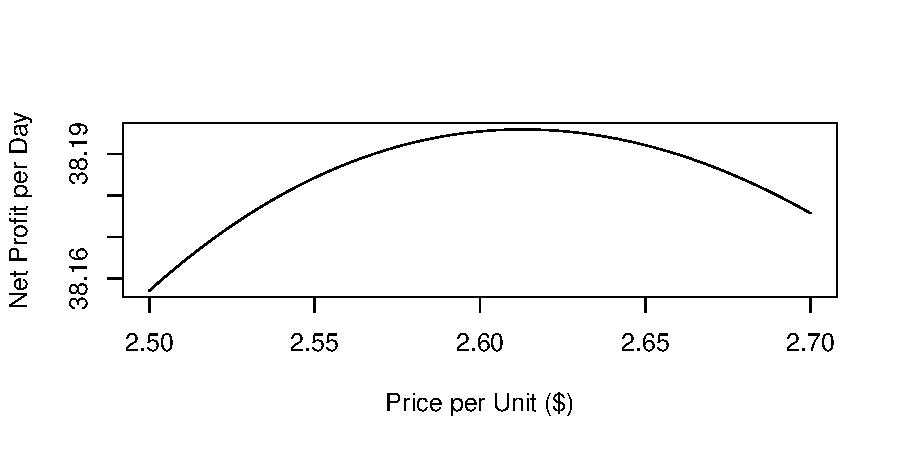
\includegraphics{Report_files/figure-latex/milk7-1.pdf}

Plotting these curves and zooming into the region where the global
maximum lies, we can observe that the function peaks at approximately
\(P = 2.61\). Thus, we should charge a price of \$2.61 per unit in order
obtain a maximum profit of approximately \$38.20 per day.

\end{document}
